%%% TeX-master: "manuscript"
% !TeX spellcheck=en_GB

\newpage

\section*{Figure Legends}

\subsection*{Figure 1}

\begin{figure}[ht]
  \centering
  \includegraphics{fig_1_pathway_overview}
  \caption{\textbf{Schematic overview of NAD biosynthesis pathways.} NAD can be synthesised from tryptophan (Trp), nicotinamide (Nam), nicotinic acid (NA), and to a lesser extend nicotinamide ribose (NR). Nam is the main precursor in human and also the product of NAD-consuming signalling reactions by enzymes such as sirtuins (NAD-dependent deacylases) or PARPs (poly-ADP-ribosylases). For the recycling of Nam, two different pathways exist. The pathway found in yeast, plants, and many bacteria starts with the deamidation of Nam by Nam deamidase (NADA). The other three enzymes comprise the Preiss-Handler pathway that also exists in vertebrates. The pathway found in vertebrates directly converts Nam into the corresponding mononucleotide (NMN) by the Nam phosphoribosyltransferase (NamPT). The Nam N-methyltransferase (NNMT) degrades Nam to methyl-Nam (MNam), which is in mammals excreted with the urine.}
  \label{fig:pathway_overview}
\end{figure}

\newpage


\subsection*{Figure 2}

\begin{figure}[ht]
  \centering
  \includegraphics[width=0.75\textwidth]{fig_2_phylo_distribution}
  \caption{\textbf{Phylogenetic distribution of NADA, NNMT, and NamPT and their relation to the number of NAD consumers.} A) Distribution of NADA, NNMT, and NamPT in selected clades. NADA is dominant in bacteria, fungi, and plants (Viridiplantae), whereas NamPT together with NNMT is dominant in Metazoa. Numbers at the pie charts show, how many species of the clades possess the respective enzyme combination indicated by the colour explained in the lower right of the figure. The number of species in a clade is given below its name. B) Common tree of selected clades within the Metazoa, including 334 species. The pie charts indicate the distribution of species within the respective clade that encode the enzyme combination indicated by the different colours. The size of the pie charts is proportional to the logarithm of the number of species analysed in the particular clade. The numbers below the clade names indicate the average number of NAD-consuming enzyme families found in all species of that clade. The branch length is arbitrary.}
  \label{fig:phylo_distribution}
\end{figure}

\newpage


\subsection*{Figure 3}

\begin{figure}[ht]
  \centering
  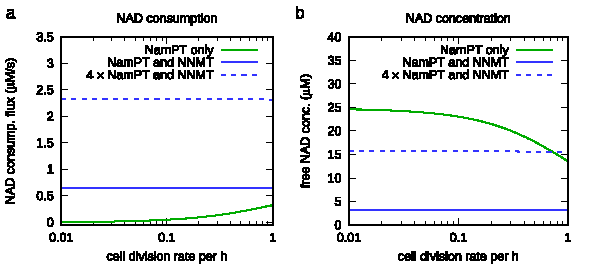
\includegraphics[width=\textwidth]{fig_3_NNMT_NAD_flux}
  \caption{\textbf{NNMT enables high NAD consumption flux.} We used a dynamic model of NAD biosynthesis and consumption (for details, see Experimental Procedures) to simulate steady state NAD consumption flux (A) and concentration (B). The amount of NMNAT and NamPT used in the simulations where adjusted such that the free NAD concentrations were in the range reported in the literature. All other enzyme concentrations were set equal. Details are given in supplementary table~S2. In the presence of NNMT (blue lines), steady state NAD consumption rates are higher despite reduced NAD concentrations. Increasing the amount of NamPT in the simulation fourfold (blue dotted lines) partially compensates for the decreased NAD concentration caused by Nam degradation through NNMT.}
  \label{fig:NNMT_NAD_flux}
\end{figure}

\newpage


\subsection*{Figure 4}

\begin{figure}[ht]
  \centering
  \includegraphics[width=0.72\textwidth]{fig_4_NamPT_affinity_Nam}
  \caption{\textbf{Role of NamPT substrate affinity.} We simulated the effect of different Michaelis-Menten constants ($K_{M}$) of NamPT for Nam on the steady state NAD consumption flux and NAD concentration at different cell division rates. All parameters were equal to those used for the simulations in figure~\ref{fig:NNMT_NAD_flux}. In the absence of NNMT, the $K_{M}$ of NamPT has little influence on NAD consumption (A) and concentration (B), but both are strongly influenced by cell division rates. In the presence of NNMT, decreasing $K_{M}$ of NamPT enables increasing NAD consumption flux (C) and NAD concentration (D). NNMT furthermore makes both, NAD consumption flux and concentration, almost independent of cell division rates. Comparing the situation with and without NNMT (E and F) at two different NamPT $K_{M}$ values reveals that at high $K_{M}$ (dashed lines) and high cell division rates NNMT no longer enables higher NAD consumption rates compared to NamPT alone (green line and dashed grey line).}
  \label{fig:NamPT_affinity_Nam}
\end{figure}

\newpage


\subsection*{Figure 5}

\begin{figure}[ht]
  \centering
  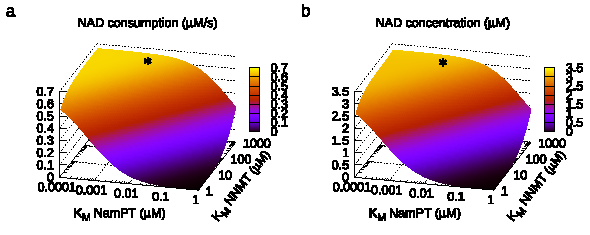
\includegraphics[width=\textwidth]{fig_5_optimal_substr_affinities}
  \caption{\textbf{The substrate affinities of human NNMT and NamPT are close to optimum.} We simulated the impact of changes in the $K_{M}$ for both NamPT and NNMT on NAD consumption rates (A) and NAD concentration (B). Both are increasing with decreasing $K_{M}$ of NamPT, but increasing $K_{M}$ of NNMT. The affinities reported for human enzymes (indicated by a black asterisk) appear to be close to the theoretical optimum, as further improvements would have little effect on NAD consumption or concentration.}
  \label{fig:optimal_substr_affinities}
\end{figure}

\newpage


\subsection*{Figure 6}

\begin{figure}[ht]
  \centering
  \includegraphics[width=0.7\textwidth]{fig_6_unresolved_loop}
  \caption{\textbf{The function of the structurally unresolved loop of NamPT.} Most deuterostomes that possess NamPT and NNMT show a sequence insertion in the N-terminal region of NamPT that has been revealed by multiple sequence alignment of NamPT from different species (A). Coloured circles indicate the enzymes present in the respective species; blue: NamPT and NNMT; black: NamPT, NADA and NNMT; yellow: NamPT and NADA. For a more comprehensive alignment, please see supplementary figure~S1. The structure visualisation of human NamPT (B) is based on a structure prediction by SWISS-MODEL \cite{Arnold2006,Biasini2014} using the model 2H3D of the human NamPT as template \cite{Wang2006}. The inserted region is not resolved in any of currently available crystal structures of NamPT and thus appears to be a flexible loop structure at the surface of the NamPT dimer, coloured in red. Immunofluorescence images (C) show that the localisation of the FLAG-tagged mutant protein lacking the unresolved loop is not changed compared to FLAG-tagged human wildtype NamPT. Both show a heterogeneous nuclear-cytosolic localisation in HeLa S3 cells. \textit{In vitro} measurements using recombinant protein show that the mutant NamPT has a lower activity than the wildtype enzyme (D) and is not activated by ATP (E). Bars in panels D and E that have different letters indicate significant difference of measured values as estimated using a T~test assuming independent samples and significance at $p < 0.05$.}
  \label{fig:unresolved_loop}
\end{figure}

\newpage


\subsection*{Figure 7}

\begin{figure}[ht]
  \centering
  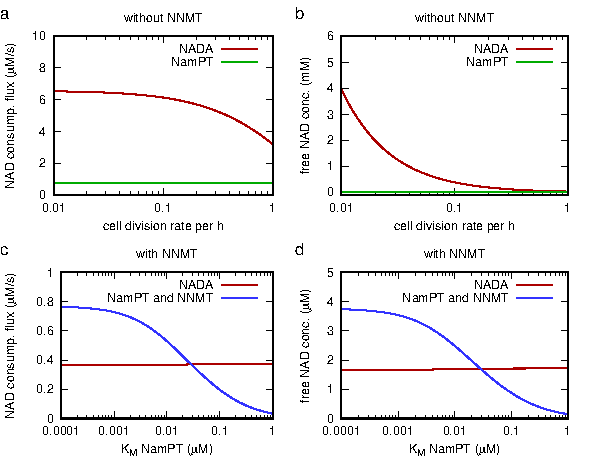
\includegraphics[width=\textwidth]{fig_7_NNMT_comp_advantage}
  \caption{\textbf{NNMT provides a competitive advantage and makes NADA obsolete.} To simulate competition for common resources, we created a two-compartment model where one compartment contained NADA, but no NamPT and the other compartment contained NamPT either with or without NNMT, but no NADA. NADA and NamPT were simulated to be present at equal amounts. In the absence of NNMT the compartment containing NADA has slightly lower NAD consumption rates (A), but much higher steady state NAD concentrations (B). In the presence of NNMT, however, both NAD consumption (C) and NAD concentration (D) are lower in the NADA compartment. This effect is dependent on a low NamPT $K_{M}$.}
  \label{fig:NNMT_comp_advantage}
\end{figure}

\newpage


\subsection*{Figure 8}

\begin{figure}[ht]
  \centering
  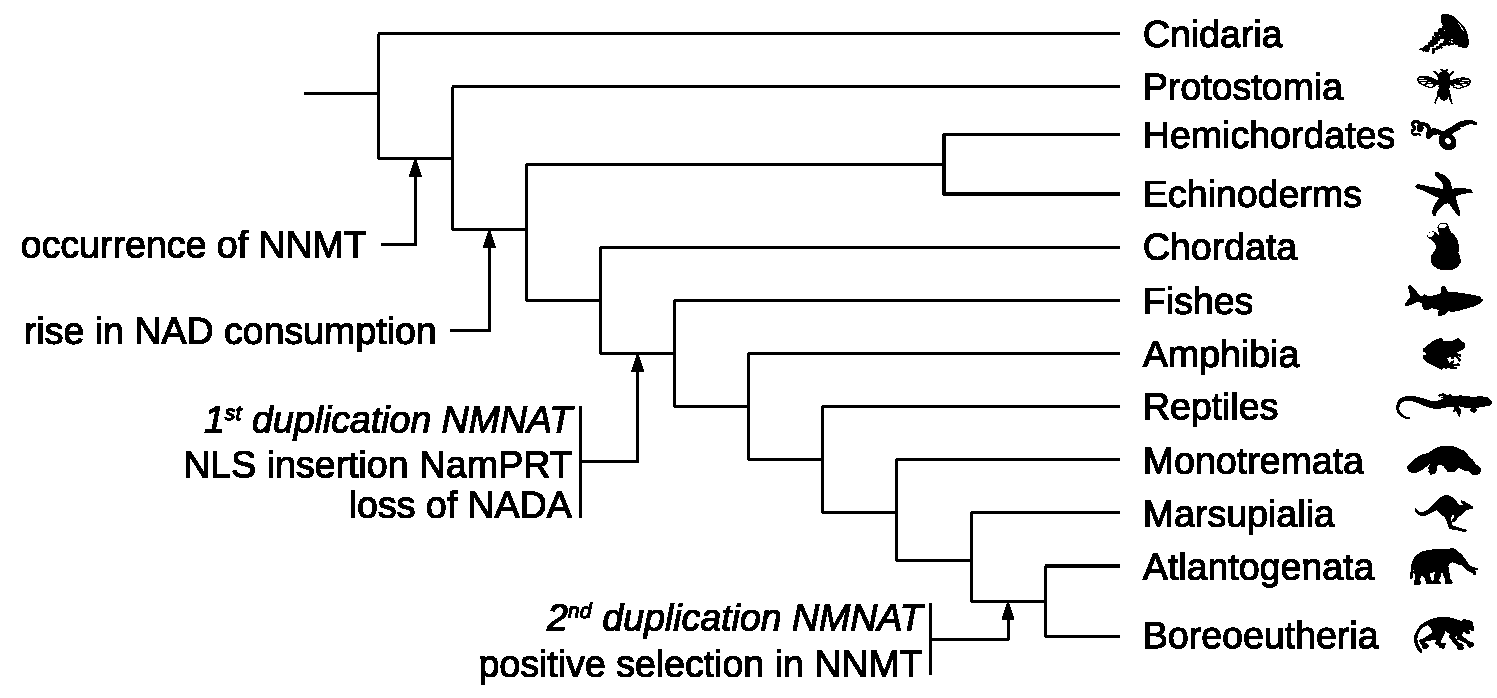
\includegraphics[width=\textwidth]{fig_8_evo_events}
  \caption{\textbf{Schematic representation of evolutionary events in the NAD pathway.} Based on the phylogenetic analysis presented here (roman font) and earlier work \cite{Lau2010} (italic font) we summarised and indicated important events in the evolution of NAD metabolism in Metazoa.}
  \label{fig:evo_events}
\end{figure}
